% !TEX root = ../main.tex
%

\section{Results}
\label{sec:results}


\subsection{Main findings}
\label{ssec:results:main}

\paragraph{Finding 1: LLM facilitators significantly improve synthetic discussions over time.} Unmoderated discussions tend to display significantly higher levels of toxicity (Fig.~\ref{fig:toxicity_stats}, Table~\ref{tab:toxicity}). A linear regression analysis of toxicity over time ($Adj. R^2 = 0.413$) reveals that trolls exhibit intense toxicity---on average $1.3288$ points above neutral users and $1.3112$ above community veterans ($p < .000$) which decreases by an average of $\minus0.0125$ points per turn ($p = 0.003$). This trend is even more pronounced for neutral participants and community veterans, whose toxicity drops by $\minus0.0225$ ($p < .000$) and $\minus0.0350$ ($p < .000$) points per turn, respectively. This demonstrates the ability of the facilitator to reign in discussions over time, but also the diverging behaviors of different roles.

\begin{figure}
	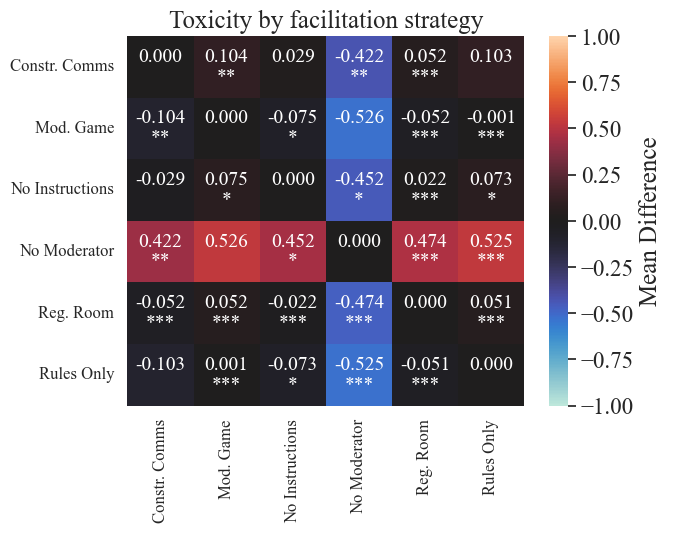
\includegraphics[width=\linewidth]{toxicity_stats.png}
	\centering
	\caption{Difference in average toxicity levels for comments following pairs of facilitation strategies. Red cells ($x>0$) indicate that the strategy on the left performs worse than the one on the bottom, for an average of $x$ points in a scale of 1-5. Conversely for blue ($x<0$) cells. White cells denote minute changes. Asterisks derived from pairwise Student-t tests (\asterisknote). The large size of our dataset allows using parametric tests.}
	\label{fig:toxicity_stats}
\end{figure}

\paragraph{Finding 2: Elaborate facilitation strategies fail to decrease toxicity.}
The real-life strategies and our own strategy (\S\ref{ssec:experimental:strategies}) show a slight edge over time compared to \emph{\strategynoinstr}, but they do not consistently outperform it (Fig~\ref{fig:toxicity_stats}). This suggests that out-of-the-box LLMs may struggle to meaningfully incorporate complex instructions---which has been noted in prior work \cite{cho-etal-2024-language}.

\begin{table}[t]
	\centering
	\begin{tabular}{p{5cm} p{1.5cm}}
		\toprule
		\textbf{Variable} & \textbf{Toxicity} \\
		\midrule
		Intercept & 2.164\textsuperscript{***} \\
		\strategynoinstr & -0.426\textsuperscript{***} \\
		\strategymodgame & -0.435\textsuperscript{***} \\
		\strategyrules & -0.461\textsuperscript{***} \\
		\strategyregroom & -0.277\textsuperscript{***} \\
		\strategyconstrcomm & -0.230\textsuperscript{***} \\
		time & -0.012\textsuperscript{**} \\
		\strategynoinstr$\times$time & -0.003 \\
		\strategymodgame$\times$time & -0.011\textsuperscript{*} \\
		\strategyrules$\times$time & -0.008 \\
		\strategyregroom$\times$time & -0.023\textsuperscript{***} \\
		\strategyconstrcomm$\times$time & -0.023\textsuperscript{***} \\
		\bottomrule
	\end{tabular}
	\small
	\asterisknote
	\normalsize
	\caption{OLS regression coefficients for toxicity on the non-facilitator comments ($Adj. R^2=0.054$). Reference factor is \textit{\strategynomod}. All strategies outperform \textit{\strategynomod} in general. The \textit{\strategyregroom} and \textit{\strategyconstrcomm} real-life strategies additionally show improvements over time compared to \textit{\strategynoinstr}.}
	\label{tab:toxicity}
\end{table}


\paragraph{Finding 3: LLM facilitators choose to intervene far too frequently, which is tolerated by the other participants.} Fig.~\ref{fig:intervention_count} demonstrates that LLM facilitators intervene at almost any opportunity, even though they are instructed to only do so when necessary. This confirms that LLMs generally can not decide not to speak even when instructed to do so  (\S\ref{ssec:methodology:us}). To our knowledge, this has not been reported in relevant literature, and \emph{is an example of ``debugging'' problems with LLMs} --- a core motivation of our work.

Additionally, we note that LLM participants exhibit atypical tolerance for excessive facilitator interventions. Humans in contrast typically become irritated and more toxic after repeated, unneeded interventions \citep{schaffner_community_guidelines, make_reddit_great, proactive_moderation, cresci_pesonalized_interventions}. This is likely another artifact of LLMs being too agreeable \citep{park2023game, anthis_2025}.

\begin{figure}[t]
	\centering
	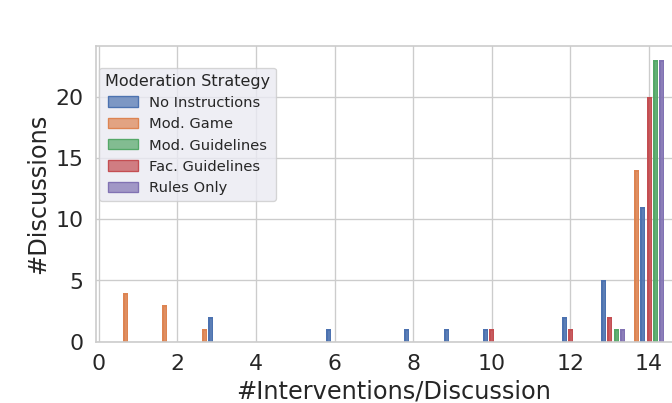
\includegraphics[width=\columnwidth]{intervention_count.png}
	\caption{Histogram of interventions by LLM facilitators per strategy used.}
	\label{fig:intervention_count}
\end{figure}


\subsection{Ablation Study}
\label{ssec:results:ablation}

\begin{figure*}[t]
    \begin{subfigure}{0.32\linewidth}
        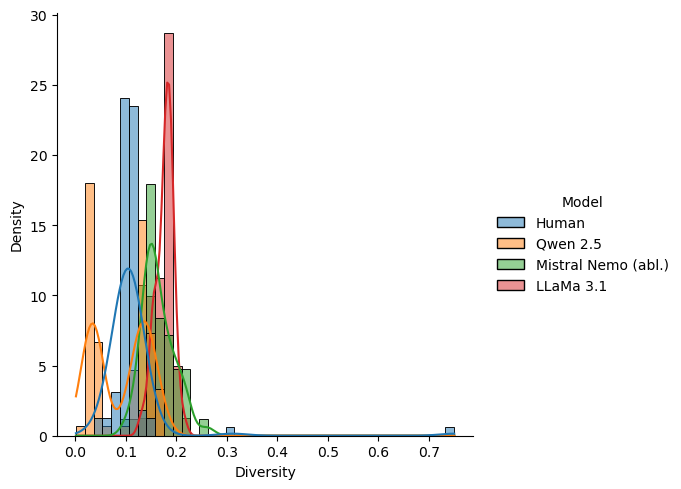
\includegraphics[width=\textwidth]{rougel_model.png}
        \caption{Model}
        \label{fig:rougel_model}
    \end{subfigure}%
    \hfill
    \begin{subfigure}{0.32\linewidth}
        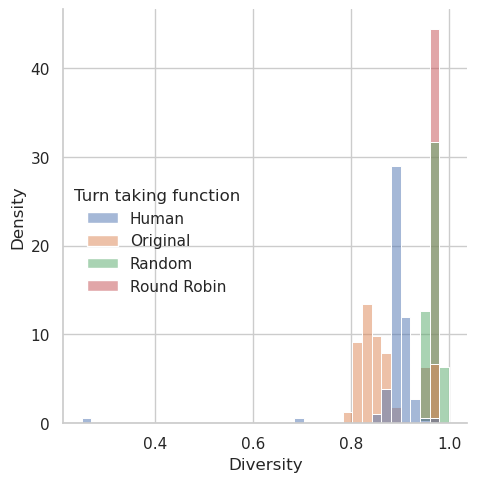
\includegraphics[width=\textwidth]{rougel_turns.png}
        \caption{Turn-taking function}
        \label{fig:rougel_turns}
    \end{subfigure}%
    \hfill
    \begin{subfigure}{0.32\linewidth}
        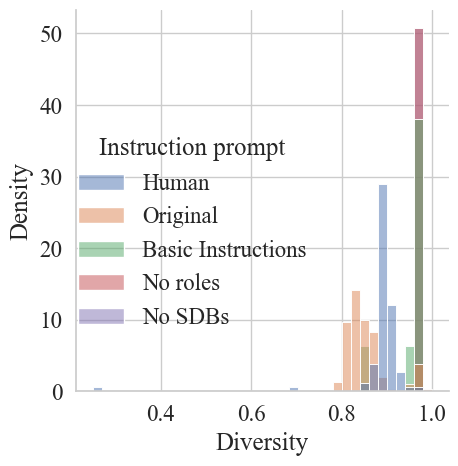
\includegraphics[width=\textwidth]{rougel_prompts.png}
        \caption{Instruction prompt}
        \label{fig:rougel_prompts}
    \end{subfigure}%

    \caption{Diversity (\S\ref{ssec:related:quality}) distribution for each discussion by LLM (\S\ref{ssec:experimental:setup}), turn-taking function $t$, and prompting function $\phi$ used (\S\ref{ssec:methodology:us}). Comparison with the CeRI Regulation Room dataset (``Human''). Note that the x-axis starts from $0.6$.}
    \label{fig:diversity}
\end{figure*}

\begin{figure}[t]
	\centering
	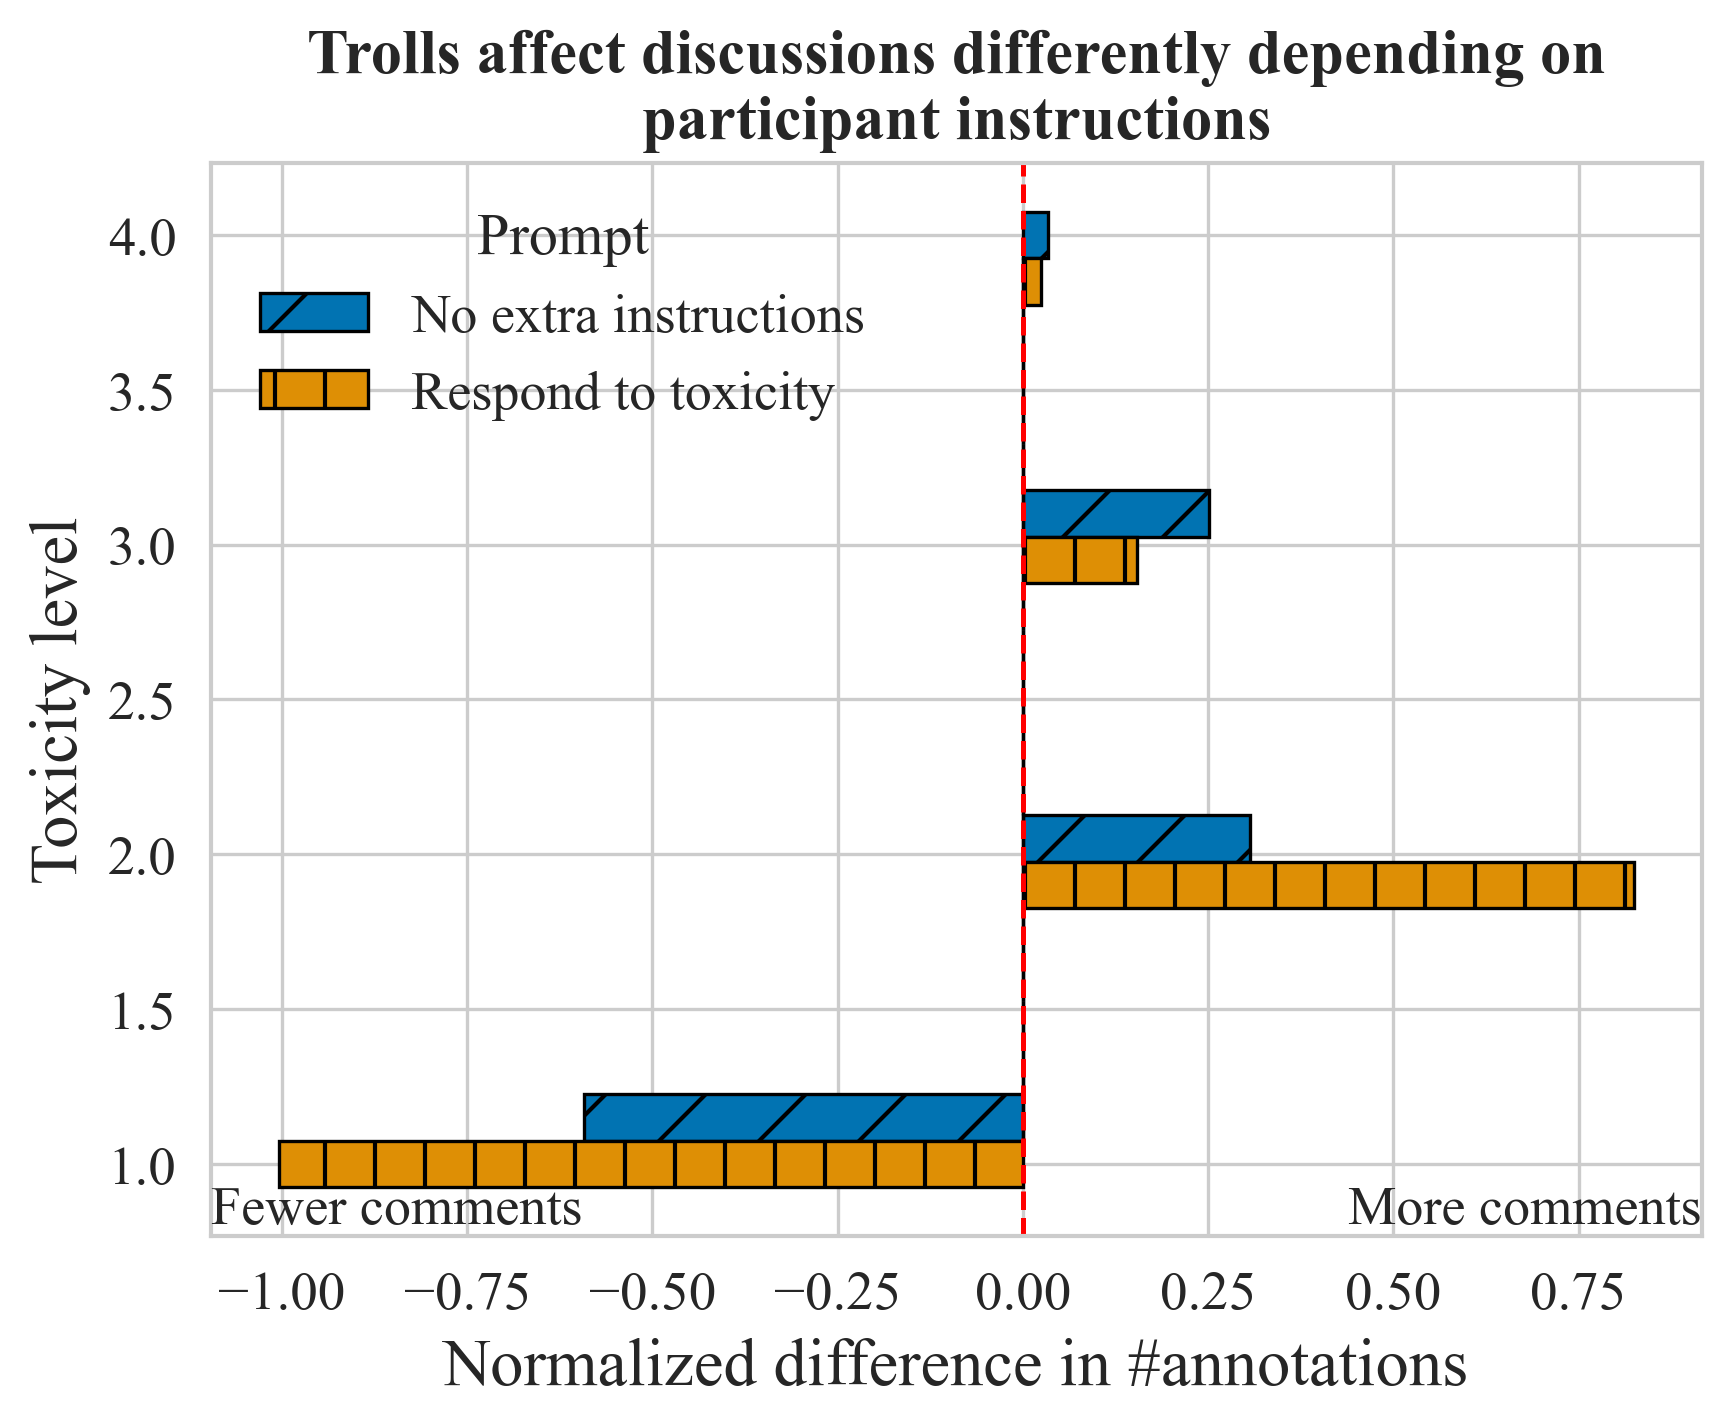
\includegraphics[width=0.8\linewidth]{toxicity_trolls.png}
	\caption{Non-troll toxicity levels in discussions with and without trolls. There is a significant uptick on the number of ``somewhat toxic" ($Toxicity=2$) comments when the participants are instructed to respond to toxic comments.}
	\label{fig:toxicity_trolls}
\end{figure}

We generate eight synthetic discussions per ablation experiment, using a single model (Qwen 2.5). We compare the diversity (cf. \S\ref{ssec:related:quality}, \S\ref{ssec:experimental:evaluation}) of these discussions with our broader synthetic dataset, as well as the CeRI “Regulation Room” dataset.\footnote{Disclaimer: Any opinions, findings, and conclusions or recommendations expressed in this material are those of the author(s) and do not necessarily reflect the views of the CeRI.} We pick this dataset because it is publicly available and comprised of facilitated online human discussions on ten diverse topics.

\paragraph{Each component of our methodology surpasses baselines in data quality.} We compare our turn-taking function (\S\ref{ssec:methodology:us}) to two baselines: Round Robin (participants speaking one after the other, then repeating) and Random Selection (uniformly sampling another participant each turn). Fig.~\ref{fig:rougel_turns} demonstrates that although all distributions diverge from the human distribution, our function is the only one not exhibiting extremely high diversity (i.e., very limited participant interaction \S\ref{ssec:experimental:evaluation}). Fig.~\ref{fig:rougel_prompts} illustrates that each individual prompting design decision (SDBs, roles, and instruction prompts) results in diversity scores more closely aligned with human discussions.

\paragraph{Larger models do not increase the quality of discussions.} As shown in Fig.~\ref{fig:rougel_model}, Qwen demonstrated the highest diversity among the evaluated models, indicating limited participant interaction (\S\ref{ssec:related:quality}), followed by Mistral Nemo and LLaMa. It's worth noting that none of the models closely matched the diversity observed in human discussions. 

\paragraph{Specialized instruction prompts are essential for eliciting toxic behavior in instruction-tuned LLMs.} Inserting trolls into the discussion leads to more intense toxicity among \emph{other} participants \emph{only if we instruct them to react to toxic posts} (Fig.~\ref{fig:toxicity_trolls}). 

